\documentclass[a4paper]{book}
\usepackage{makeidx}
\usepackage{natbib}
\usepackage{graphicx}
\usepackage{multicol}
\usepackage{float}
\usepackage{listings}
\usepackage{color}
\usepackage{ifthen}
\usepackage[table]{xcolor}
\usepackage{textcomp}
\usepackage{alltt}
\usepackage{ifpdf}
\ifpdf
\usepackage[pdftex,
            pagebackref=true,
            colorlinks=true,
            linkcolor=blue,
            unicode
           ]{hyperref}
\else
\usepackage[ps2pdf,
            pagebackref=true,
            colorlinks=true,
            linkcolor=blue,
            unicode
           ]{hyperref}
\usepackage{pspicture}
\fi
\usepackage[utf8]{inputenc}
\usepackage{mathptmx}
\usepackage[scaled=.90]{helvet}
\usepackage{courier}
\usepackage{sectsty}
\usepackage[titles]{tocloft}
\usepackage{doxygen}
\lstset{language=C++,inputencoding=utf8,basicstyle=\footnotesize,breaklines=true,breakatwhitespace=true,tabsize=4,numbers=left }
\makeindex
\setcounter{tocdepth}{3}
\renewcommand{\footrulewidth}{0.4pt}
\renewcommand{\familydefault}{\sfdefault}
\hfuzz=15pt
\setlength{\emergencystretch}{15pt}
\hbadness=750
\tolerance=750
\begin{document}
\hypersetup{pageanchor=false,citecolor=blue}
\begin{titlepage}
\vspace*{7cm}
\begin{center}
{\Large \-Frugal \-Distributed \-Media \-Network }\\
\vspace*{1cm}
{\large \-Generated by Doxygen 1.7.6.1}\\
\vspace*{0.5cm}
{\small Fri Feb 10 2012 11:32:22}\\
\end{center}
\end{titlepage}
\clearemptydoublepage
\pagenumbering{roman}
\tableofcontents
\clearemptydoublepage
\pagenumbering{arabic}
\hypersetup{pageanchor=true,citecolor=blue}
\chapter{\-Class \-Index}
\section{\-Class \-Hierarchy}
\-This inheritance list is sorted roughly, but not completely, alphabetically\-:\begin{DoxyCompactList}
\item \contentsline{section}{\-Attr\-Vector}{\pageref{d0/d39/classAttrVector}}{}
\item \contentsline{section}{c\-Core\-Module}{\pageref{d7/d7b/classcCoreModule}}{}
\begin{DoxyCompactList}
\item \contentsline{section}{c\-F\-D\-M\-N\-Protocol}{\pageref{d7/d9d/classcFDMNProtocol}}{}
\item \contentsline{section}{c\-Net\-Interface}{\pageref{da/de4/classcNetInterface}}{}
\item \contentsline{section}{c\-Settings}{\pageref{d0/d75/classcSettings}}{}
\end{DoxyCompactList}
\item \contentsline{section}{c\-I\-D\-\_\-dispatch}{\pageref{d6/d70/classcID__dispatch}}{}
\item \contentsline{section}{c\-Log}{\pageref{d9/d47/classcLog}}{}
\item \contentsline{section}{c\-Mount\-Info}{\pageref{d7/d18/classcMountInfo}}{}
\item \contentsline{section}{c\-Mount\-Sys}{\pageref{d8/dfe/classcMountSys}}{}
\item \contentsline{section}{c\-Protocol}{\pageref{d0/dfe/classcProtocol}}{}
\begin{DoxyCompactList}
\item \contentsline{section}{c\-F\-D\-M\-N\-Protocol}{\pageref{d7/d9d/classcFDMNProtocol}}{}
\end{DoxyCompactList}
\item \contentsline{section}{c\-Server\-Core}{\pageref{d7/d07/classcServerCore}}{}
\item \contentsline{section}{node}{\pageref{d5/da1/structnode}}{}
\item \contentsline{section}{\-Options\-Base}{\pageref{d0/d13/classOptionsBase}}{}
\begin{DoxyCompactList}
\item \contentsline{section}{mount\-Options}{\pageref{da/db5/classmountOptions}}{}
\end{DoxyCompactList}
\item \contentsline{section}{packet}{\pageref{df/de8/structpacket}}{}
\item \contentsline{section}{queue\-\_\-t}{\pageref{da/de4/structqueue__t}}{}
\item \contentsline{section}{\-S\-T\-A\-T\-\_\-packet}{\pageref{d0/d26/structSTAT__packet}}{}
\item \contentsline{section}{ts\-\_\-queue}{\pageref{d8/dc0/structts__queue}}{}
\item \contentsline{section}{u\-Option}{\pageref{d9/d8f/structuOption}}{}
\end{DoxyCompactList}

\chapter{\-Class \-Index}
\section{\-Class \-List}
\-Here are the classes, structs, unions and interfaces with brief descriptions\-:\begin{DoxyCompactList}
\item\contentsline{section}{\hyperlink{classAttrVector}{\-Attr\-Vector} }{\pageref{d0/d39/classAttrVector}}{}
\item\contentsline{section}{\hyperlink{classcCoreModule}{c\-Core\-Module} }{\pageref{d7/d7b/classcCoreModule}}{}
\item\contentsline{section}{\hyperlink{classcFDMNProtocol}{c\-F\-D\-M\-N\-Protocol} }{\pageref{d7/d9d/classcFDMNProtocol}}{}
\item\contentsline{section}{\hyperlink{classcID__dispatch}{c\-I\-D\-\_\-dispatch} }{\pageref{d6/d70/classcID__dispatch}}{}
\item\contentsline{section}{\hyperlink{classcLog}{c\-Log} }{\pageref{d9/d47/classcLog}}{}
\item\contentsline{section}{\hyperlink{classcMountInfo}{c\-Mount\-Info} }{\pageref{d7/d18/classcMountInfo}}{}
\item\contentsline{section}{\hyperlink{classcMountSys}{c\-Mount\-Sys} }{\pageref{d8/dfe/classcMountSys}}{}
\item\contentsline{section}{\hyperlink{classcNetInterface}{c\-Net\-Interface} }{\pageref{da/de4/classcNetInterface}}{}
\item\contentsline{section}{\hyperlink{classcProtocol}{c\-Protocol} }{\pageref{d0/dfe/classcProtocol}}{}
\item\contentsline{section}{\hyperlink{classcServerCore}{c\-Server\-Core} }{\pageref{d7/d07/classcServerCore}}{}
\item\contentsline{section}{\hyperlink{classcSettings}{c\-Settings} }{\pageref{d0/d75/classcSettings}}{}
\item\contentsline{section}{\hyperlink{classmountOptions}{mount\-Options} }{\pageref{da/db5/classmountOptions}}{}
\item\contentsline{section}{\hyperlink{structnode}{node} }{\pageref{d5/da1/structnode}}{}
\item\contentsline{section}{\hyperlink{classOptionsBase}{\-Options\-Base} }{\pageref{d0/d13/classOptionsBase}}{}
\item\contentsline{section}{\hyperlink{structpacket}{packet} }{\pageref{df/de8/structpacket}}{}
\item\contentsline{section}{\hyperlink{structqueue__t}{queue\-\_\-t} }{\pageref{da/de4/structqueue__t}}{}
\item\contentsline{section}{\hyperlink{structSTAT__packet}{\-S\-T\-A\-T\-\_\-packet} }{\pageref{d0/d26/structSTAT__packet}}{}
\item\contentsline{section}{\hyperlink{structts__queue}{ts\-\_\-queue} }{\pageref{d8/dc0/structts__queue}}{}
\item\contentsline{section}{\hyperlink{structuOption}{u\-Option} }{\pageref{d9/d8f/structuOption}}{}
\end{DoxyCompactList}

\chapter{\-Class \-Documentation}
\hypertarget{classAttrVector}{\section{\-Attr\-Vector \-Class \-Reference}
\label{d0/d39/classAttrVector}\index{\-Attr\-Vector@{\-Attr\-Vector}}
}
\subsection*{\-Public \-Member \-Functions}
\begin{DoxyCompactItemize}
\item 
\hypertarget{classAttrVector_ad275d0597a50822974e652947c101fbf}{vector$<$ file\-Attrs $>$ \& {\bfseries get\-Vector} ()}\label{d0/d39/classAttrVector_ad275d0597a50822974e652947c101fbf}

\end{DoxyCompactItemize}


\-The documentation for this class was generated from the following files\-:\begin{DoxyCompactItemize}
\item 
include/file\-\_\-management/fs\-\_\-util.\-h\item 
src/file\-\_\-management/fs\-\_\-util.\-cpp\end{DoxyCompactItemize}

\hypertarget{classcCoreModule}{\section{c\-Core\-Module \-Class \-Reference}
\label{d7/d7b/classcCoreModule}\index{c\-Core\-Module@{c\-Core\-Module}}
}
\-Inheritance diagram for c\-Core\-Module\-:\begin{figure}[H]
\begin{center}
\leavevmode
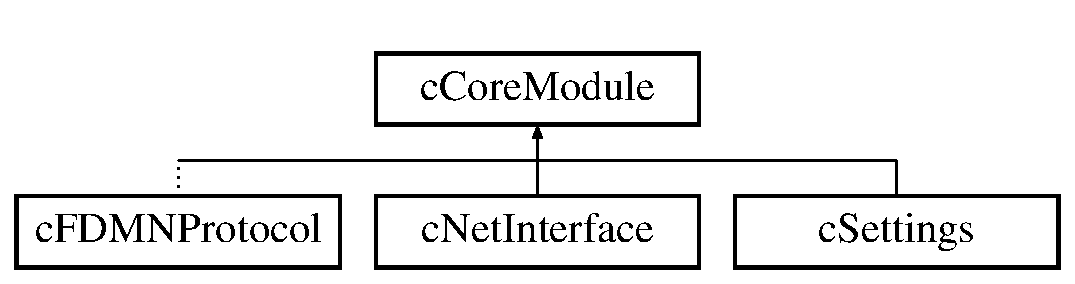
\includegraphics[height=2.000000cm]{d7/d7b/classcCoreModule}
\end{center}
\end{figure}
\subsection*{\-Public \-Member \-Functions}
\begin{DoxyCompactItemize}
\item 
\hypertarget{classcCoreModule_ada5a543231ca01861d76e49d6fbd97d9}{virtual void {\bfseries status} (stringstream \&)=0}\label{d7/d7b/classcCoreModule_ada5a543231ca01861d76e49d6fbd97d9}

\item 
\hypertarget{classcCoreModule_ade87c33167c935b211aa70cd3591ad6a}{virtual void {\bfseries cleanup} ()=0}\label{d7/d7b/classcCoreModule_ade87c33167c935b211aa70cd3591ad6a}

\end{DoxyCompactItemize}


\-The documentation for this class was generated from the following file\-:\begin{DoxyCompactItemize}
\item 
include/core\-\_\-classes.\-h\end{DoxyCompactItemize}

\hypertarget{classcFDMNProtocol}{\section{c\-F\-D\-M\-N\-Protocol \-Class \-Reference}
\label{d7/d9d/classcFDMNProtocol}\index{c\-F\-D\-M\-N\-Protocol@{c\-F\-D\-M\-N\-Protocol}}
}
\-Inheritance diagram for c\-F\-D\-M\-N\-Protocol\-:\begin{figure}[H]
\begin{center}
\leavevmode
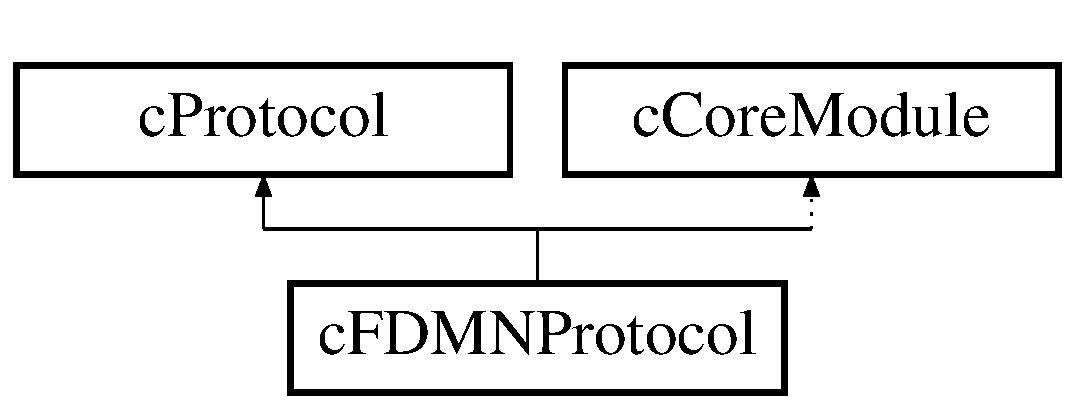
\includegraphics[height=2.000000cm]{d7/d9d/classcFDMNProtocol}
\end{center}
\end{figure}
\subsection*{\-Public \-Member \-Functions}
\begin{DoxyCompactItemize}
\item 
\hypertarget{classcFDMNProtocol_a39964d16ee56e37c020fa82665b52831}{void {\bfseries init\-\_\-mappings} ()}\label{d7/d9d/classcFDMNProtocol_a39964d16ee56e37c020fa82665b52831}

\item 
\hypertarget{classcFDMNProtocol_a5a1475b1b4cb6fc548bb9879a2bfee11}{void {\bfseries init\-Queue} ()}\label{d7/d9d/classcFDMNProtocol_a5a1475b1b4cb6fc548bb9879a2bfee11}

\item 
\hypertarget{classcFDMNProtocol_ab7f40203a9fc3564100dc96ec55429d4}{void {\bfseries start\-Threads} ()}\label{d7/d9d/classcFDMNProtocol_ab7f40203a9fc3564100dc96ec55429d4}

\item 
\hypertarget{classcFDMNProtocol_a7c00ee18ee000d08d6de92a3166c44d9}{void {\bfseries listen} ()}\label{d7/d9d/classcFDMNProtocol_a7c00ee18ee000d08d6de92a3166c44d9}

\item 
\hypertarget{classcFDMNProtocol_ab1e32cb3c94a8932030e40f4841aa9b7}{void {\bfseries add\-Msg} (int)}\label{d7/d9d/classcFDMNProtocol_ab1e32cb3c94a8932030e40f4841aa9b7}

\item 
\hypertarget{classcFDMNProtocol_aea7f1aa23979f8a79830d65b08988eaf}{void {\bfseries status} (stringstream \&stream)}\label{d7/d9d/classcFDMNProtocol_aea7f1aa23979f8a79830d65b08988eaf}

\item 
\hypertarget{classcFDMNProtocol_aac11ecb86235973a957d683d67b6da0e}{void {\bfseries cleanup} ()}\label{d7/d9d/classcFDMNProtocol_aac11ecb86235973a957d683d67b6da0e}

\end{DoxyCompactItemize}


\-The documentation for this class was generated from the following files\-:\begin{DoxyCompactItemize}
\item 
include/net\-\_\-interface.\-h\item 
src/net\-\_\-interface.\-cpp\end{DoxyCompactItemize}

\hypertarget{classcID__dispatch}{\section{c\-I\-D\-\_\-dispatch \-Class \-Reference}
\label{d6/d70/classcID__dispatch}\index{c\-I\-D\-\_\-dispatch@{c\-I\-D\-\_\-dispatch}}
}
\subsection*{\-Public \-Member \-Functions}
\begin{DoxyCompactItemize}
\item 
\hypertarget{classcID__dispatch_affdaa11979bcf753e94f5461d43821c3}{{\bfseries c\-I\-D\-\_\-dispatch} (int limit)}\label{d6/d70/classcID__dispatch_affdaa11979bcf753e94f5461d43821c3}

\item 
\hypertarget{classcID__dispatch_a0c2006cbdee6c1fa049d4d56ca1cf162}{int {\bfseries \-I\-D\-\_\-getid} ()}\label{d6/d70/classcID__dispatch_a0c2006cbdee6c1fa049d4d56ca1cf162}

\item 
\hypertarget{classcID__dispatch_a6c6907c20eadbfa7a20e9e6d6d770524}{int {\bfseries \-I\-D\-\_\-getid\-\_\-ts} ()}\label{d6/d70/classcID__dispatch_a6c6907c20eadbfa7a20e9e6d6d770524}

\item 
\hypertarget{classcID__dispatch_aa70e7c3637506ce6fa031ffb55b33665}{int {\bfseries \-I\-D\-\_\-recall} ()}\label{d6/d70/classcID__dispatch_aa70e7c3637506ce6fa031ffb55b33665}

\item 
\hypertarget{classcID__dispatch_accbab0ee78ff00a74fdff3317b24dd90}{void {\bfseries \-I\-D\-\_\-returnid} (int id)}\label{d6/d70/classcID__dispatch_accbab0ee78ff00a74fdff3317b24dd90}

\item 
\hypertarget{classcID__dispatch_a4c9874c076f685bf5a497d0741a190c6}{void {\bfseries \-I\-D\-\_\-returnid\-\_\-ts} (int id)}\label{d6/d70/classcID__dispatch_a4c9874c076f685bf5a497d0741a190c6}

\end{DoxyCompactItemize}


\-The documentation for this class was generated from the following files\-:\begin{DoxyCompactItemize}
\item 
include/utility.\-h\item 
src/utility.\-cpp\end{DoxyCompactItemize}

\hypertarget{classcLog}{\section{c\-Log \-Class \-Reference}
\label{d9/d47/classcLog}\index{c\-Log@{c\-Log}}
}
\subsection*{\-Public \-Member \-Functions}
\begin{DoxyCompactItemize}
\item 
\hypertarget{classcLog_a7e87269960564d10330a177edd1d2050}{{\bfseries c\-Log} (string filename)}\label{d9/d47/classcLog_a7e87269960564d10330a177edd1d2050}

\item 
\hypertarget{classcLog_a49f4252b9052482227bf3a7392c3bbec}{void {\bfseries log\-\_\-simple} (string message)}\label{d9/d47/classcLog_a49f4252b9052482227bf3a7392c3bbec}

\item 
\hypertarget{classcLog_a61e765767ed99591a411a0b1d9de8b9f}{void {\bfseries log\-\_\-color} (string message, const term\-Opts options\mbox{[}$\,$\mbox{]})}\label{d9/d47/classcLog_a61e765767ed99591a411a0b1d9de8b9f}

\item 
\hypertarget{classcLog_a63a0f720e95812a8176c6636001e3e79}{void {\bfseries log\-\_\-block\-\_\-msg} (string block\-\_\-msg)}\label{d9/d47/classcLog_a63a0f720e95812a8176c6636001e3e79}

\item 
\hypertarget{classcLog_a68a0fcfdb189284028f6fec5d437ae8c}{void {\bfseries toggle\-\_\-time} (bool setting)}\label{d9/d47/classcLog_a68a0fcfdb189284028f6fec5d437ae8c}

\end{DoxyCompactItemize}


\-The documentation for this class was generated from the following files\-:\begin{DoxyCompactItemize}
\item 
include/logging.\-h\item 
src/logging.\-cpp\end{DoxyCompactItemize}

\hypertarget{classcMountInfo}{\section{c\-Mount\-Info \-Class \-Reference}
\label{d7/d18/classcMountInfo}\index{c\-Mount\-Info@{c\-Mount\-Info}}
}
\subsection*{\-Public \-Member \-Functions}
\begin{DoxyCompactItemize}
\item 
\hypertarget{classcMountInfo_ad41825c13091e499df3606f36477ce8d}{vector$<$ file\-Attrs $>$ \& {\bfseries get\-Attrs} ()}\label{d7/d18/classcMountInfo_ad41825c13091e499df3606f36477ce8d}

\item 
\hypertarget{classcMountInfo_a60c0c7efcc06de43aee97c098f7ca79e}{void {\bfseries add\-Regular} (\hyperlink{classcMountInfo}{c\-Mount\-Info} $\ast$)}\label{d7/d18/classcMountInfo_a60c0c7efcc06de43aee97c098f7ca79e}

\item 
\hypertarget{classcMountInfo_a504cafc1098657ecbd2f3523d02297c8}{void {\bfseries add\-Dir} (\hyperlink{classcMountInfo}{c\-Mount\-Info} $\ast$)}\label{d7/d18/classcMountInfo_a504cafc1098657ecbd2f3523d02297c8}

\item 
\hypertarget{classcMountInfo_a456f1229fe86b8815f738bd174e4409a}{void {\bfseries print\-Content} (int indent\-Lvl=0)}\label{d7/d18/classcMountInfo_a456f1229fe86b8815f738bd174e4409a}

\item 
\hypertarget{classcMountInfo_a922916b79833982f1196cdd9709e5970}{int {\bfseries number\-Files} (e\-File\-Type)}\label{d7/d18/classcMountInfo_a922916b79833982f1196cdd9709e5970}

\item 
\hypertarget{classcMountInfo_a57176c82a28af7af249c1d5913387dc7}{filesystem\-::path \& {\bfseries get\-Path} ()}\label{d7/d18/classcMountInfo_a57176c82a28af7af249c1d5913387dc7}

\end{DoxyCompactItemize}
\subsection*{\-Static \-Public \-Member \-Functions}
\begin{DoxyCompactItemize}
\item 
\hypertarget{classcMountInfo_a73d0efc6da4fd3c07acd9a8e500faac4}{static void {\bfseries set\-Path} (\hyperlink{classcMountInfo}{c\-Mount\-Info} \&, string path)}\label{d7/d18/classcMountInfo_a73d0efc6da4fd3c07acd9a8e500faac4}

\item 
\hypertarget{classcMountInfo_a8bbce14d7375ba7c09e7b30ee19bbe3a}{static void {\bfseries set\-Path} (\hyperlink{classcMountInfo}{c\-Mount\-Info} \&, filesystem\-::path path)}\label{d7/d18/classcMountInfo_a8bbce14d7375ba7c09e7b30ee19bbe3a}

\item 
\hypertarget{classcMountInfo_aa3fa521adbe386fa8a327b515ae15d6f}{static void {\bfseries set\-Size} (\hyperlink{classcMountInfo}{c\-Mount\-Info} \&, ssize\-\_\-t size)}\label{d7/d18/classcMountInfo_aa3fa521adbe386fa8a327b515ae15d6f}

\item 
\hypertarget{classcMountInfo_a0ac01041a1f7e65a23e138033fb8c4d8}{static void {\bfseries set\-Type} (\hyperlink{classcMountInfo}{c\-Mount\-Info} \&, e\-File\-Type type)}\label{d7/d18/classcMountInfo_a0ac01041a1f7e65a23e138033fb8c4d8}

\item 
\hypertarget{classcMountInfo_a5bc9493c54685a90b96525b5dbee7d4d}{static \hyperlink{classcMountInfo}{c\-Mount\-Info} $\ast$ {\bfseries add\-File} (\hyperlink{classcMountInfo}{c\-Mount\-Info} \&, e\-File\-Type)}\label{d7/d18/classcMountInfo_a5bc9493c54685a90b96525b5dbee7d4d}

\item 
\hypertarget{classcMountInfo_a4a8965b26d3cc92610de7f0db164c057}{static void {\bfseries sort\-Mounts} (\hyperlink{classcMountInfo}{c\-Mount\-Info} \&)}\label{d7/d18/classcMountInfo_a4a8965b26d3cc92610de7f0db164c057}

\end{DoxyCompactItemize}
\subsection*{\-Public \-Attributes}
\begin{DoxyCompactItemize}
\item 
\hypertarget{classcMountInfo_a5ccfba3b945fa785dcae4c22e655e804}{e\-File\-Type {\bfseries entry\-Type}}\label{d7/d18/classcMountInfo_a5ccfba3b945fa785dcae4c22e655e804}

\item 
\hypertarget{classcMountInfo_ab7a61cb3c40f4222f290d161260d37e1}{filesystem\-::path {\bfseries entry\-Path}}\label{d7/d18/classcMountInfo_ab7a61cb3c40f4222f290d161260d37e1}

\item 
\hypertarget{classcMountInfo_ac4145e903e7a5668c49e40113476482c}{ssize\-\_\-t {\bfseries entry\-Size}}\label{d7/d18/classcMountInfo_ac4145e903e7a5668c49e40113476482c}

\end{DoxyCompactItemize}
\subsection*{\-Static \-Protected \-Member \-Functions}
\begin{DoxyCompactItemize}
\item 
\hypertarget{classcMountInfo_aa847892a0fc2fe52a39173c2e95ffd33}{static void {\bfseries print\-Indent} (int level)}\label{d7/d18/classcMountInfo_aa847892a0fc2fe52a39173c2e95ffd33}

\end{DoxyCompactItemize}
\subsection*{\-Protected \-Attributes}
\begin{DoxyCompactItemize}
\item 
\hypertarget{classcMountInfo_a02b0f7b087f44acc08d5259d870111b5}{vector$<$ \hyperlink{classcMountInfo}{c\-Mount\-Info} $\ast$ $>$ {\bfseries regular\-Files}}\label{d7/d18/classcMountInfo_a02b0f7b087f44acc08d5259d870111b5}

\item 
\hypertarget{classcMountInfo_abccd2011842fec9fbde9bd2fff28e17e}{vector$<$ \hyperlink{classcMountInfo}{c\-Mount\-Info} $\ast$ $>$ {\bfseries directories}}\label{d7/d18/classcMountInfo_abccd2011842fec9fbde9bd2fff28e17e}

\end{DoxyCompactItemize}


\-The documentation for this class was generated from the following files\-:\begin{DoxyCompactItemize}
\item 
include/file\-\_\-management/fs\-\_\-util.\-h\item 
src/file\-\_\-management/fs\-\_\-util.\-cpp\end{DoxyCompactItemize}

\hypertarget{classcMountSys}{\section{c\-Mount\-Sys \-Class \-Reference}
\label{d8/dfe/classcMountSys}\index{c\-Mount\-Sys@{c\-Mount\-Sys}}
}
\subsection*{\-Public \-Member \-Functions}
\begin{DoxyCompactItemize}
\item 
\hypertarget{classcMountSys_a495ef5e6d5743705d2be4f5a1c14c4b5}{void {\bfseries set\-Root} (string \&)}\label{d8/dfe/classcMountSys_a495ef5e6d5743705d2be4f5a1c14c4b5}

\item 
\hypertarget{classcMountSys_a705f723af4efcf73271787ab61dacd99}{bool {\bfseries new\-Mount} (string location)}\label{d8/dfe/classcMountSys_a705f723af4efcf73271787ab61dacd99}

\item 
\hypertarget{classcMountSys_adcd5ee25a58026dab99c25ac0bc12523}{void {\bfseries print\-Mounts} ()}\label{d8/dfe/classcMountSys_adcd5ee25a58026dab99c25ac0bc12523}

\end{DoxyCompactItemize}


\-The documentation for this class was generated from the following files\-:\begin{DoxyCompactItemize}
\item 
include/file\-\_\-management/mounts.\-h\item 
src/file\-\_\-management/mounts.\-cpp\end{DoxyCompactItemize}

\hypertarget{classcNetInterface}{\section{c\-Net\-Interface \-Class \-Reference}
\label{da/de4/classcNetInterface}\index{c\-Net\-Interface@{c\-Net\-Interface}}
}
\-Inheritance diagram for c\-Net\-Interface\-:\begin{figure}[H]
\begin{center}
\leavevmode
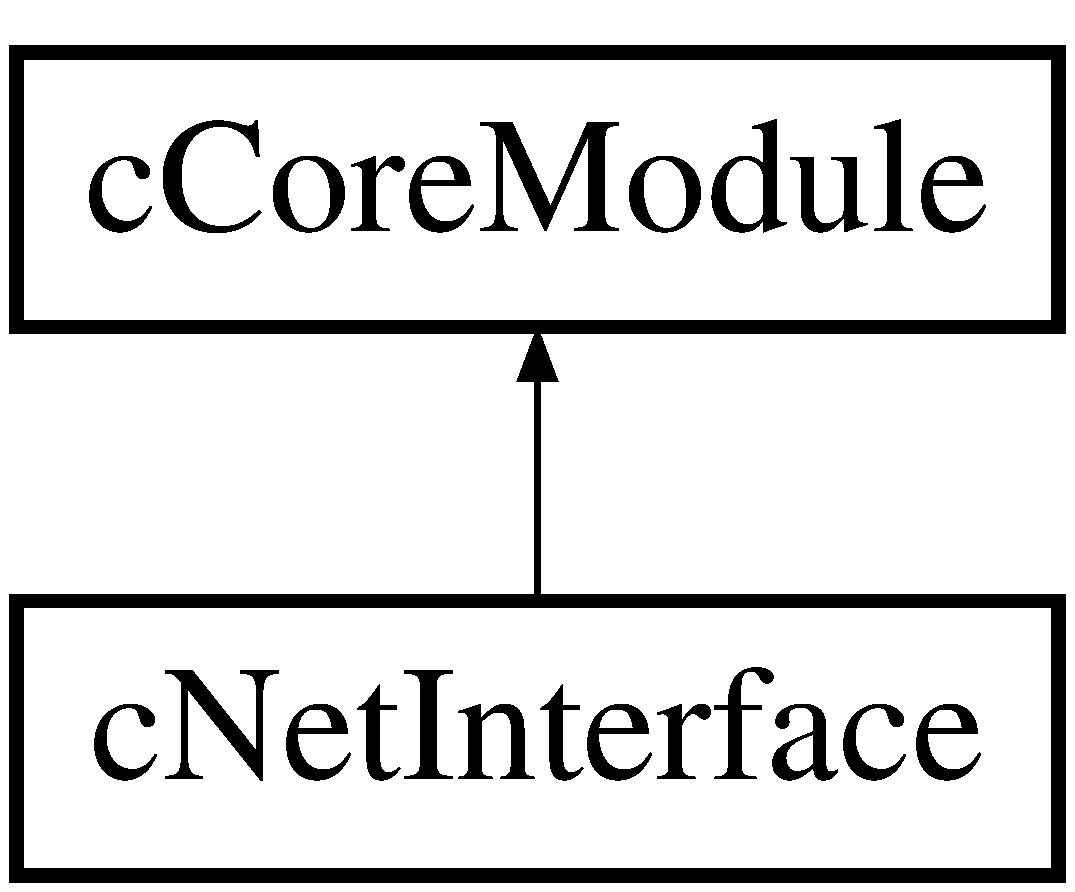
\includegraphics[height=2.000000cm]{da/de4/classcNetInterface}
\end{center}
\end{figure}
\subsection*{\-Public \-Member \-Functions}
\begin{DoxyCompactItemize}
\item 
\hypertarget{classcNetInterface_a7b38cb9a362e729b8ef73245f9991fc2}{{\bfseries c\-Net\-Interface} (int port)}\label{da/de4/classcNetInterface_a7b38cb9a362e729b8ef73245f9991fc2}

\item 
\hypertarget{classcNetInterface_acea432f78242bb6edcb8f81a30114d1e}{void {\bfseries init\-\_\-net} (int port)}\label{da/de4/classcNetInterface_acea432f78242bb6edcb8f81a30114d1e}

\item 
\hypertarget{classcNetInterface_ad50e432a498ed9d24a58ef0390bbd983}{void {\bfseries set\-\_\-protocol} (\hyperlink{classcProtocol}{c\-Protocol} $\ast$)}\label{da/de4/classcNetInterface_ad50e432a498ed9d24a58ef0390bbd983}

\item 
\hypertarget{classcNetInterface_ab732d7b5c74093909877a2b4447cb9b2}{void {\bfseries start\-\_\-listening} ()}\label{da/de4/classcNetInterface_ab732d7b5c74093909877a2b4447cb9b2}

\item 
\hypertarget{classcNetInterface_a1005c326968e4e1cff622200a434d329}{void {\bfseries status} (stringstream \&stream)}\label{da/de4/classcNetInterface_a1005c326968e4e1cff622200a434d329}

\item 
\hypertarget{classcNetInterface_a29518e90ddc07c2ba44e6df688af0fe7}{void {\bfseries cleanup} ()}\label{da/de4/classcNetInterface_a29518e90ddc07c2ba44e6df688af0fe7}

\end{DoxyCompactItemize}


\-The documentation for this class was generated from the following files\-:\begin{DoxyCompactItemize}
\item 
include/net\-\_\-interface.\-h\item 
src/net\-\_\-interface.\-cpp\end{DoxyCompactItemize}

\hypertarget{classcProtocol}{\section{c\-Protocol \-Class \-Reference}
\label{d0/dfe/classcProtocol}\index{c\-Protocol@{c\-Protocol}}
}
\-Inheritance diagram for c\-Protocol\-:\begin{figure}[H]
\begin{center}
\leavevmode
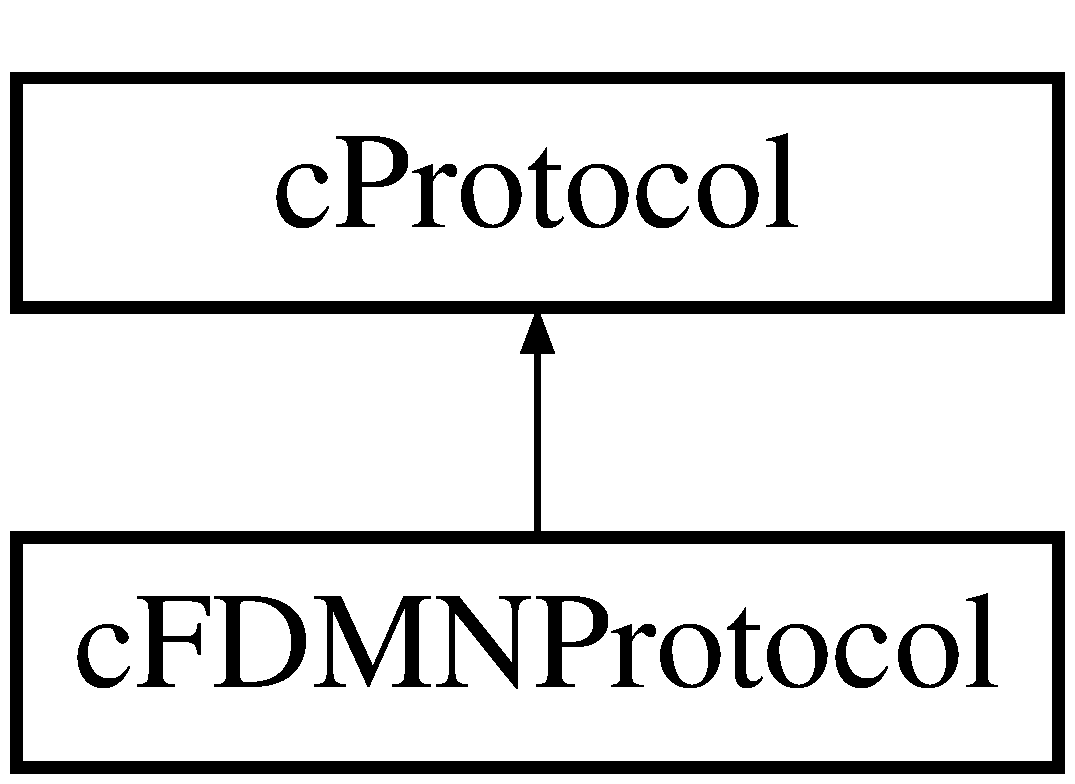
\includegraphics[height=2.000000cm]{d0/dfe/classcProtocol}
\end{center}
\end{figure}
\subsection*{\-Public \-Member \-Functions}
\begin{DoxyCompactItemize}
\item 
\hypertarget{classcProtocol_ad3acd1123c6379a82c4b42fa9ad68d4b}{virtual void {\bfseries add\-Msg} (int)=0}\label{d0/dfe/classcProtocol_ad3acd1123c6379a82c4b42fa9ad68d4b}

\end{DoxyCompactItemize}


\-The documentation for this class was generated from the following files\-:\begin{DoxyCompactItemize}
\item 
include/net\-\_\-interface.\-h\item 
src/net\-\_\-interface.\-cpp\end{DoxyCompactItemize}

\hypertarget{classcServerCore}{\section{c\-Server\-Core \-Class \-Reference}
\label{d7/d07/classcServerCore}\index{c\-Server\-Core@{c\-Server\-Core}}
}
\subsection*{\-Public \-Member \-Functions}
\begin{DoxyCompactItemize}
\item 
\hypertarget{classcServerCore_accc35f76d7064522fb8483465a34d117}{{\bfseries c\-Server\-Core} (string settings\-\_\-file)}\label{d7/d07/classcServerCore_accc35f76d7064522fb8483465a34d117}

\item 
\hypertarget{classcServerCore_ae6d720ebdc88a47cd82ef9701e1f24e3}{void {\bfseries cleanup} ()}\label{d7/d07/classcServerCore_ae6d720ebdc88a47cd82ef9701e1f24e3}

\item 
\hypertarget{classcServerCore_a7c38faeb17d1bf9705c65082ef7d9e35}{void {\bfseries start\-\_\-server} ()}\label{d7/d07/classcServerCore_a7c38faeb17d1bf9705c65082ef7d9e35}

\item 
\hypertarget{classcServerCore_ad2d7490392221f486c05dfcdade9a5a5}{void {\bfseries status} (uint32\-\_\-t flags, bool log)}\label{d7/d07/classcServerCore_ad2d7490392221f486c05dfcdade9a5a5}

\end{DoxyCompactItemize}
\subsection*{\-Static \-Public \-Member \-Functions}
\begin{DoxyCompactItemize}
\item 
\hypertarget{classcServerCore_a9cc302f6c83a40f646b78d3b9f03c31c}{static string {\bfseries version} ()}\label{d7/d07/classcServerCore_a9cc302f6c83a40f646b78d3b9f03c31c}

\end{DoxyCompactItemize}


\-The documentation for this class was generated from the following files\-:\begin{DoxyCompactItemize}
\item 
include/server\-\_\-core.\-h\item 
src/server\-\_\-core.\-cpp\end{DoxyCompactItemize}

\hypertarget{classcSettings}{\section{c\-Settings \-Class \-Reference}
\label{d0/d75/classcSettings}\index{c\-Settings@{c\-Settings}}
}
\-Inheritance diagram for c\-Settings\-:\begin{figure}[H]
\begin{center}
\leavevmode
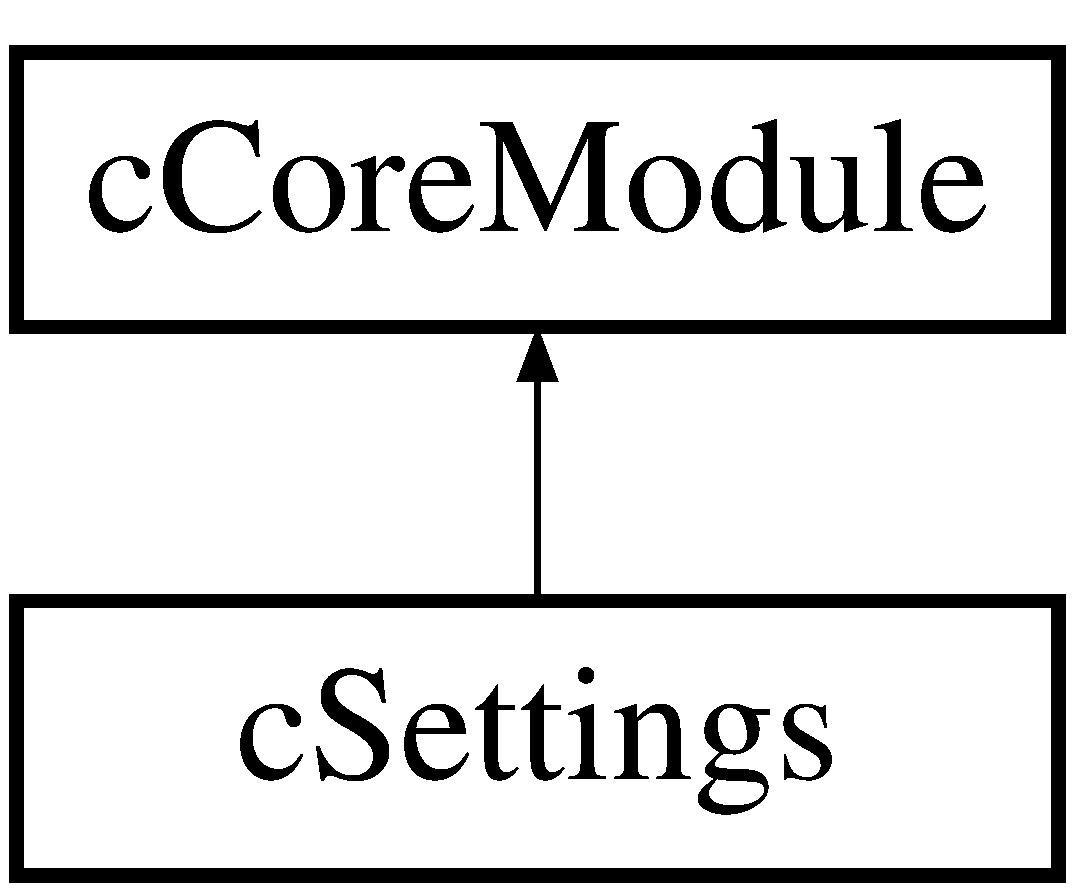
\includegraphics[height=2.000000cm]{d0/d75/classcSettings}
\end{center}
\end{figure}
\subsection*{\-Public \-Member \-Functions}
\begin{DoxyCompactItemize}
\item 
\hypertarget{classcSettings_adb4191f32f2bed59d41bcc4c5d0c6317}{{\bfseries c\-Settings} (\-I\-N\-I\-Reader $\ast$ini)}\label{d0/d75/classcSettings_adb4191f32f2bed59d41bcc4c5d0c6317}

\item 
\hypertarget{classcSettings_aa2d6863d9a56f599b592e4834663dec2}{{\bfseries c\-Settings} (string filename)}\label{d0/d75/classcSettings_aa2d6863d9a56f599b592e4834663dec2}

\item 
\hypertarget{classcSettings_a52944397e64f17ba57573134c7eb9c9d}{bool {\bfseries load\-\_\-settings} (string filename=\char`\"{}\char`\"{})}\label{d0/d75/classcSettings_a52944397e64f17ba57573134c7eb9c9d}

\item 
\hypertarget{classcSettings_a096489fcd36936a5b44772a56e444ac4}{void {\bfseries set\-\_\-defaults} (void($\ast$default\-\_\-fn)(\-I\-N\-I\-Reader $\ast$))}\label{d0/d75/classcSettings_a096489fcd36936a5b44772a56e444ac4}

\item 
\hypertarget{classcSettings_a932a80fa8c18894d813bf16112402f01}{bool {\bfseries exists} (const string \&section, const string \&key)}\label{d0/d75/classcSettings_a932a80fa8c18894d813bf16112402f01}

\item 
\hypertarget{classcSettings_a2a0b1ae7d7d5e60abf092bde42e3b7af}{{\footnotesize template$<$class T $>$ }\\\-T {\bfseries extract\-Value} (const string \&section, const string \&key)}\label{d0/d75/classcSettings_a2a0b1ae7d7d5e60abf092bde42e3b7af}

\item 
\hypertarget{classcSettings_a691bc81e42a54dbd1ec7212284bef316}{{\footnotesize template$<$class T $>$ }\\\-T {\bfseries extract\-Default} (const string \&section, const string \&key)}\label{d0/d75/classcSettings_a691bc81e42a54dbd1ec7212284bef316}

\item 
\hypertarget{classcSettings_ac4ba02418b3ed5b2ce2709c2e6983e5e}{void {\bfseries status} (stringstream \&stream)}\label{d0/d75/classcSettings_ac4ba02418b3ed5b2ce2709c2e6983e5e}

\item 
\hypertarget{classcSettings_a0fb4ea27171811d337c6aca9f4ed873d}{void {\bfseries status\-\_\-all} (stringstream \&stream)}\label{d0/d75/classcSettings_a0fb4ea27171811d337c6aca9f4ed873d}

\item 
\hypertarget{classcSettings_a3878b2abb4176a3ffb7c70a87c4a3ffe}{void {\bfseries cleanup} ()}\label{d0/d75/classcSettings_a3878b2abb4176a3ffb7c70a87c4a3ffe}

\end{DoxyCompactItemize}


\-The documentation for this class was generated from the following files\-:\begin{DoxyCompactItemize}
\item 
include/settings.\-h\item 
src/settings.\-cpp\end{DoxyCompactItemize}

\hypertarget{classmountOptions}{\section{mount\-Options \-Class \-Reference}
\label{da/db5/classmountOptions}\index{mount\-Options@{mount\-Options}}
}
\-Inheritance diagram for mount\-Options\-:\begin{figure}[H]
\begin{center}
\leavevmode
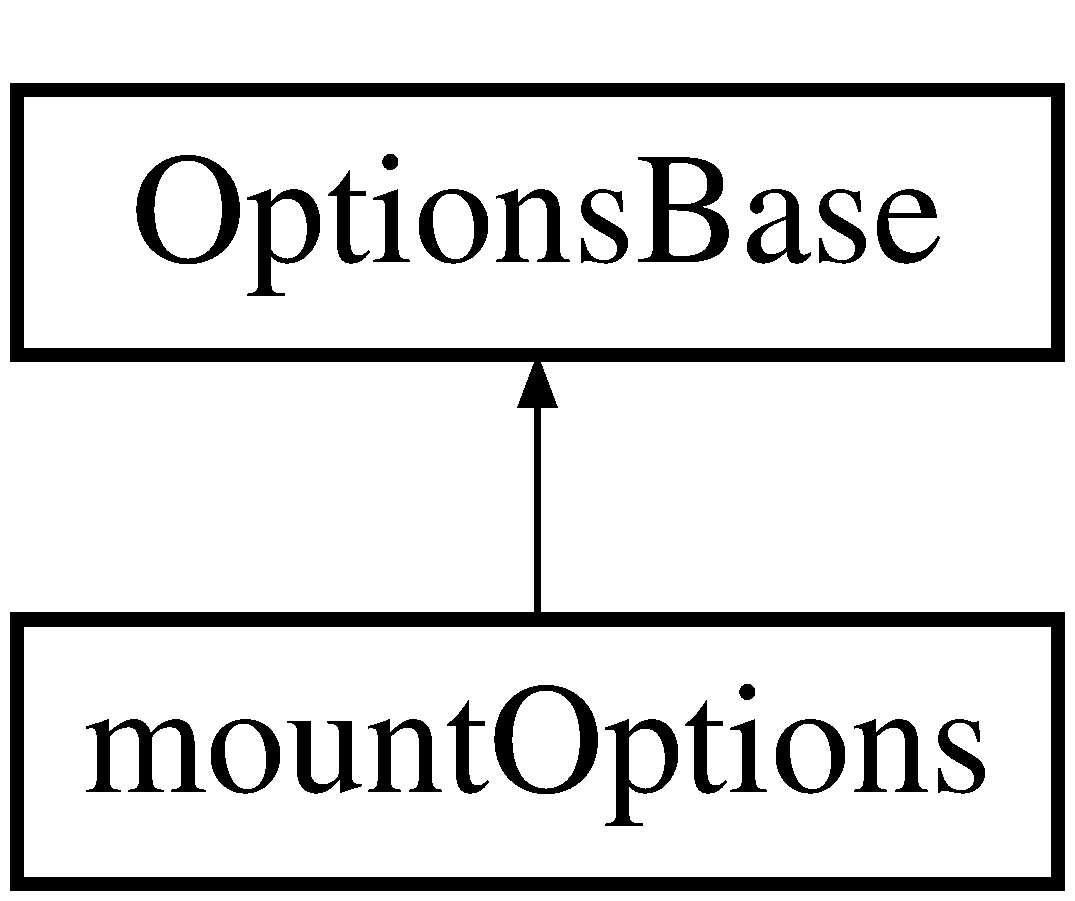
\includegraphics[height=2.000000cm]{da/db5/classmountOptions}
\end{center}
\end{figure}


\-The documentation for this class was generated from the following files\-:\begin{DoxyCompactItemize}
\item 
include/admin/cmd\-\_\-bindings/cmd\-\_\-m.\-h\item 
src/admin/cmd\-\_\-bindings/cmd\-\_\-m.\-cpp\end{DoxyCompactItemize}

\hypertarget{structnode}{\section{node \-Struct \-Reference}
\label{d5/da1/structnode}\index{node@{node}}
}
\subsection*{\-Public \-Member \-Functions}
\begin{DoxyCompactItemize}
\item 
\hypertarget{structnode_adfa3f8fbe3258d320f76c2c1065551de}{{\bfseries node} (int, \hyperlink{structnode}{node} $\ast$)}\label{d5/da1/structnode_adfa3f8fbe3258d320f76c2c1065551de}

\end{DoxyCompactItemize}
\subsection*{\-Public \-Attributes}
\begin{DoxyCompactItemize}
\item 
\hypertarget{structnode_a1df258d4663fc36cfd0d5d93588aa21f}{int {\bfseries value}}\label{d5/da1/structnode_a1df258d4663fc36cfd0d5d93588aa21f}

\item 
\hypertarget{structnode_aad210fa7c160a49f6b9a3ffee592a2bc}{\hyperlink{structnode}{node} $\ast$ {\bfseries next}}\label{d5/da1/structnode_aad210fa7c160a49f6b9a3ffee592a2bc}

\end{DoxyCompactItemize}


\-The documentation for this struct was generated from the following files\-:\begin{DoxyCompactItemize}
\item 
include/utility.\-h\item 
src/utility.\-cpp\end{DoxyCompactItemize}

\hypertarget{classOptionsBase}{\section{\-Options\-Base \-Class \-Reference}
\label{d0/d13/classOptionsBase}\index{\-Options\-Base@{\-Options\-Base}}
}
\-Inheritance diagram for \-Options\-Base\-:\begin{figure}[H]
\begin{center}
\leavevmode
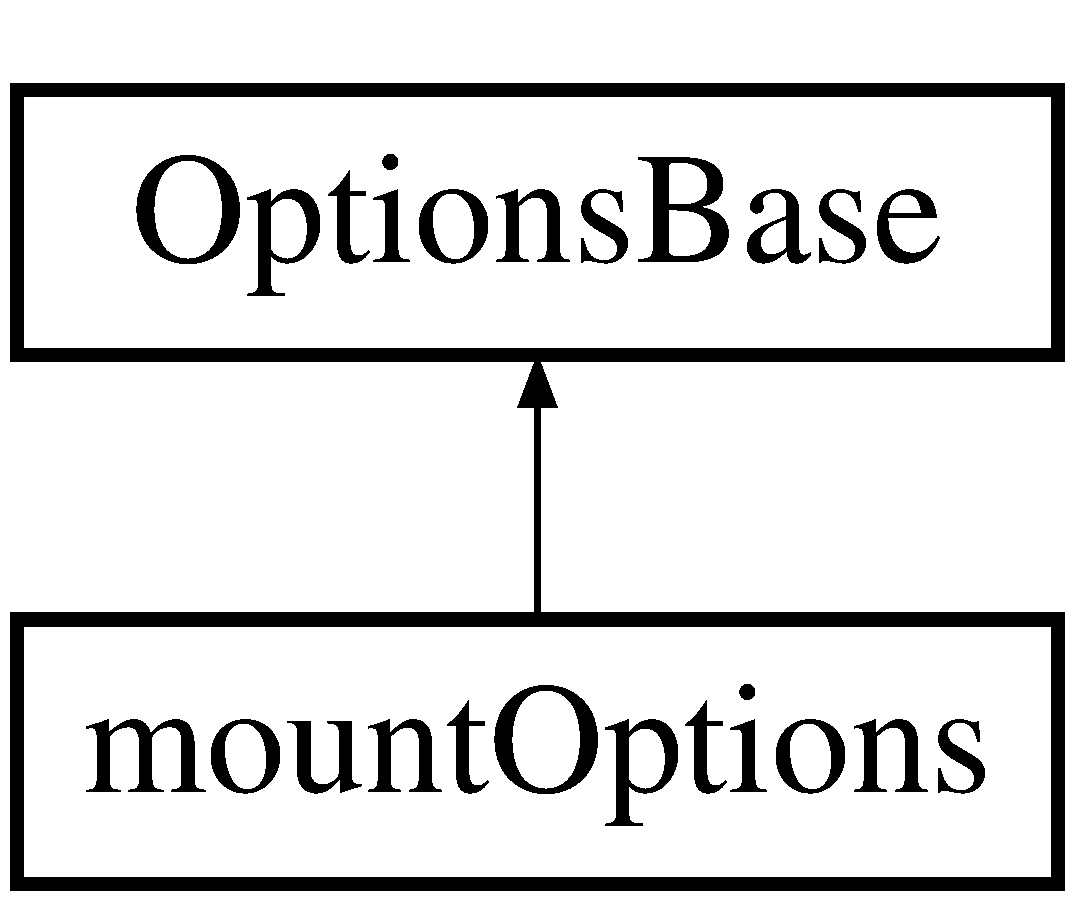
\includegraphics[height=2.000000cm]{d0/d13/classOptionsBase}
\end{center}
\end{figure}
\subsection*{\-Public \-Member \-Functions}
\begin{DoxyCompactItemize}
\item 
\hypertarget{classOptionsBase_af36ccbd9db3c53e1ec4b8163eca1bccb}{arg\-Map \& {\bfseries operator()} ()}\label{d0/d13/classOptionsBase_af36ccbd9db3c53e1ec4b8163eca1bccb}

\end{DoxyCompactItemize}
\subsection*{\-Protected \-Attributes}
\begin{DoxyCompactItemize}
\item 
\hypertarget{classOptionsBase_a230ad2f42262ae364bf1c2ef2bb70994}{arg\-Map {\bfseries options}}\label{d0/d13/classOptionsBase_a230ad2f42262ae364bf1c2ef2bb70994}

\end{DoxyCompactItemize}


\-The documentation for this class was generated from the following files\-:\begin{DoxyCompactItemize}
\item 
include/utility.\-h\item 
src/utility.\-cpp\end{DoxyCompactItemize}

\hypertarget{structpacket}{\section{packet \-Struct \-Reference}
\label{df/de8/structpacket}\index{packet@{packet}}
}
\subsection*{\-Public \-Attributes}
\begin{DoxyCompactItemize}
\item 
\hypertarget{structpacket_a89ea3290474a887d116c03acc214f7c8}{enum\-Req\-Type {\bfseries request}}\label{df/de8/structpacket_a89ea3290474a887d116c03acc214f7c8}

\item 
\hypertarget{structpacket_ad3115ffc58cc55bae08635ed965c4768}{void $\ast$ {\bfseries data}}\label{df/de8/structpacket_ad3115ffc58cc55bae08635ed965c4768}

\end{DoxyCompactItemize}


\-The documentation for this struct was generated from the following file\-:\begin{DoxyCompactItemize}
\item 
include/network/packets.\-h\end{DoxyCompactItemize}

\hypertarget{structqueue__t}{\section{queue\-\_\-t \-Struct \-Reference}
\label{da/de4/structqueue__t}\index{queue\-\_\-t@{queue\-\_\-t}}
}
\subsection*{\-Public \-Attributes}
\begin{DoxyCompactItemize}
\item 
\hypertarget{structqueue__t_ac029f683449143dfb455497c8f65be41}{int {\bfseries fd}}\label{da/de4/structqueue__t_ac029f683449143dfb455497c8f65be41}

\item 
\hypertarget{structqueue__t_a6d9023097f98241daf5e40c96a401c30}{int {\bfseries id}}\label{da/de4/structqueue__t_a6d9023097f98241daf5e40c96a401c30}

\end{DoxyCompactItemize}


\-The documentation for this struct was generated from the following file\-:\begin{DoxyCompactItemize}
\item 
include/utility.\-h\end{DoxyCompactItemize}

\hypertarget{structSTAT__packet}{\section{\-S\-T\-A\-T\-\_\-packet \-Struct \-Reference}
\label{d0/d26/structSTAT__packet}\index{\-S\-T\-A\-T\-\_\-packet@{\-S\-T\-A\-T\-\_\-packet}}
}
\subsection*{\-Public \-Attributes}
\begin{DoxyCompactItemize}
\item 
\hypertarget{structSTAT__packet_ad6962f4247e0ec11279a5c7fb681e5e7}{uint16\-\_\-t {\bfseries mount}}\label{d0/d26/structSTAT__packet_ad6962f4247e0ec11279a5c7fb681e5e7}

\item 
\hypertarget{structSTAT__packet_a700f76ff727071755a7ed52e9308adb4}{char {\bfseries filereq} \mbox{[}\-M\-A\-X\-\_\-\-P\-A\-T\-H\-S\-I\-Z\-E\mbox{]}}\label{d0/d26/structSTAT__packet_a700f76ff727071755a7ed52e9308adb4}

\end{DoxyCompactItemize}


\-The documentation for this struct was generated from the following file\-:\begin{DoxyCompactItemize}
\item 
include/network/packets.\-h\end{DoxyCompactItemize}

\hypertarget{structts__queue}{\section{ts\-\_\-queue \-Struct \-Reference}
\label{d8/dc0/structts__queue}\index{ts\-\_\-queue@{ts\-\_\-queue}}
}
\subsection*{\-Public \-Attributes}
\begin{DoxyCompactItemize}
\item 
\hypertarget{structts__queue_ad0cae9c852542a4654c5d723ba906538}{pthread\-\_\-mutex\-\_\-t {\bfseries q\-\_\-lock}}\label{d8/dc0/structts__queue_ad0cae9c852542a4654c5d723ba906538}

\item 
\hypertarget{structts__queue_a9b4bd3067a357146ba9088e6b435c8f7}{pthread\-\_\-cond\-\_\-t {\bfseries q\-\_\-full}}\label{d8/dc0/structts__queue_a9b4bd3067a357146ba9088e6b435c8f7}

\item 
\hypertarget{structts__queue_a49aff9cc7b2cffb3e9ea76e8a6ee0872}{pthread\-\_\-cond\-\_\-t {\bfseries q\-\_\-empty}}\label{d8/dc0/structts__queue_a49aff9cc7b2cffb3e9ea76e8a6ee0872}

\item 
\hypertarget{structts__queue_ab89bcdfc115f126854e2e4600d50b5d2}{int {\bfseries size}}\label{d8/dc0/structts__queue_ab89bcdfc115f126854e2e4600d50b5d2}

\item 
\hypertarget{structts__queue_a6d83dc742d44ab788272bdd459ae9e19}{int {\bfseries slots\-\_\-available}}\label{d8/dc0/structts__queue_a6d83dc742d44ab788272bdd459ae9e19}

\item 
\hypertarget{structts__queue_a6857d41af0c2acc1c08b6e11767708ff}{int {\bfseries start}}\label{d8/dc0/structts__queue_a6857d41af0c2acc1c08b6e11767708ff}

\item 
\hypertarget{structts__queue_a617541f01622f3d640230b141d8f1805}{int {\bfseries end}}\label{d8/dc0/structts__queue_a617541f01622f3d640230b141d8f1805}

\item 
\hypertarget{structts__queue_af81f6be362e410a8687c142a0671928f}{\hyperlink{structqueue__t}{queue\-\_\-t} $\ast$$\ast$ {\bfseries data}}\label{d8/dc0/structts__queue_af81f6be362e410a8687c142a0671928f}

\end{DoxyCompactItemize}


\-The documentation for this struct was generated from the following file\-:\begin{DoxyCompactItemize}
\item 
include/utility.\-h\end{DoxyCompactItemize}

\hypertarget{structuOption}{\section{u\-Option \-Struct \-Reference}
\label{d9/d8f/structuOption}\index{u\-Option@{u\-Option}}
}
\subsection*{\-Public \-Attributes}
\begin{DoxyCompactItemize}
\item 
\hypertarget{structuOption_a28d94d0ef9a65e973764306f70f4ad64}{bool {\bfseries set}}\label{d9/d8f/structuOption_a28d94d0ef9a65e973764306f70f4ad64}

\item 
\hypertarget{structuOption_adb9c94e399edb1134a74fd36586d1530}{int {\bfseries int\-Arg}}\label{d9/d8f/structuOption_adb9c94e399edb1134a74fd36586d1530}

\item 
\hypertarget{structuOption_a3295bd87dfd6b701034c4f7689907024}{int {\bfseries str\-Start}}\label{d9/d8f/structuOption_a3295bd87dfd6b701034c4f7689907024}

\item 
\hypertarget{structuOption_a21ff6586bea56187617a8f63ad8167b8}{int {\bfseries str\-Len}}\label{d9/d8f/structuOption_a21ff6586bea56187617a8f63ad8167b8}

\end{DoxyCompactItemize}


\-The documentation for this struct was generated from the following file\-:\begin{DoxyCompactItemize}
\item 
include/utility.\-h\end{DoxyCompactItemize}

\printindex
\end{document}
